Испытание на воздействие повышенной температуры среды по \ref{t_k_p} настоящих~ТУ проводят следующим образом:
%
\begin{enumerate}
	\item \dut \  помещают в камеру тепла, схему собирают в соответствии с рисунком~\ref{fig:capacity_camera};
			\begin{figure}[!htb]
			\centering
			\includegraphics[page=2]{schema}
			\begin{picdescription}
				\item \ESKDtheTitle \ \RN;
				\item \hyperref[e:multimeter]{Мультиметр \multimeter};
				\item \hyperref[e:stend]{\stend \ \stendRN};
			\end{picdescription}
			\begin{picdescription}[label={E\arabic* ---}, ref={E\arabic*}, before={\vspace{0pt}\small}]
				\item \hyperref[e:cable]{Жгут \cableRN}.
			\end{picdescription}
			\caption{Схема проверки номинальной ёмкости, номинального напряжения, автоматической защиты от глубокого разряда при воздействии климатических факторов}
			\label{fig:capacity_camera}
		\end{figure}
	\item средства измерения подготавливают к работе согласно прилагаемым к ним инструкциям по эксплуатации;
	\item производятся проверки по \treb \ настоящих~ТУ;
	\item в камере устанавливают повышенную рабочую температуру окружающей среды, указанную в~\ref{m_k_p} настоящих~ТУ; 
	\item после установления заданного значения температуры \dut \ выдерживают в камере в течение $2$~ч и производят проверки по~\treb \ настоящих~ТУ;
	\item температуру в камере повышают до повышенной рабочей кратковременной, указанной в~\ref{m_k_p} настоящих~ТУ;
	\item после прогрева \dut \ в течение $2$~ч производят проверку по \treb \ настоящих ТУ;
	\item в камере устанавливают предельную повышенную температуру окружающей среды, указанную в \ref{m_k_p} настоящих~ТУ; 
	\item после установления заданного значения температуры \dut \ выдерживают в камере в течение $6$~ч;
	\item температуру в камере понижают до повышенной рабочей;
	\item после установления заданного значения температуры \dut \ выдерживают в камере в течение $2$~ч, и производят проверки по \treb \ настоящих~ТУ;
	\item температуру  в  камере  понижают  до  нормальной  и,  после выдержки в течение $2$~ч, производят проверки по \trebafter \ настоящих~ТУ.
\end{enumerate}

\dut \  считается выдержавшим проверку по \ref{t_k_p} настоящих~ТУ, если \dut \  соответствует требованиям \treb \ настоящих~ТУ в процессе испытания и соответствует \trebafter \ настоящих~ТУ после испытания.
